\chapter{The nEDM active magnetic shielding}

\label{ch:nedm_sfc}


\section{The principle of an active magnetic shielding}
\note{This is the first time the idea of an active compensation system is introduced! Need to be slow here.}
Passive methods of shielding the magnetic field, like $\upmu$-metal shields, rely on magnetic properties of materials. In contrast, in active methods the disturbances are first detected, processed and then counteracted. It is not unlike the recently popular active-noise-cancellation headphones. Standard ones provide only passive damping of the ambient noise by covering the ears. Active ones additionally feature microphones that resolve the profile of incoming sound, which is then inverted and emitted from the speakers. The two waveforms, when overlaid, cancel.

Active magnetic field compensation systems follow the same principle. A volume, sometimes called the fiducial volume, is encircled by coils, as well as has magnetic field sensors distributed in it. It is schematically presented in Fig.\,\ref{fig:sfc-scheme}: the fiducial volume is the violet structure in the middle, encircled by green dots depicting the magnetic field sensors. Around it there are three perpendicular Helmholtz-like pairs of coils, depicted in shades of orange. Variations of the magnetic field are detected by the sensors and processed to obtain the counteracting measure. The output signals are amplified and sent into the coils.

\begin{figure}
  \centering
  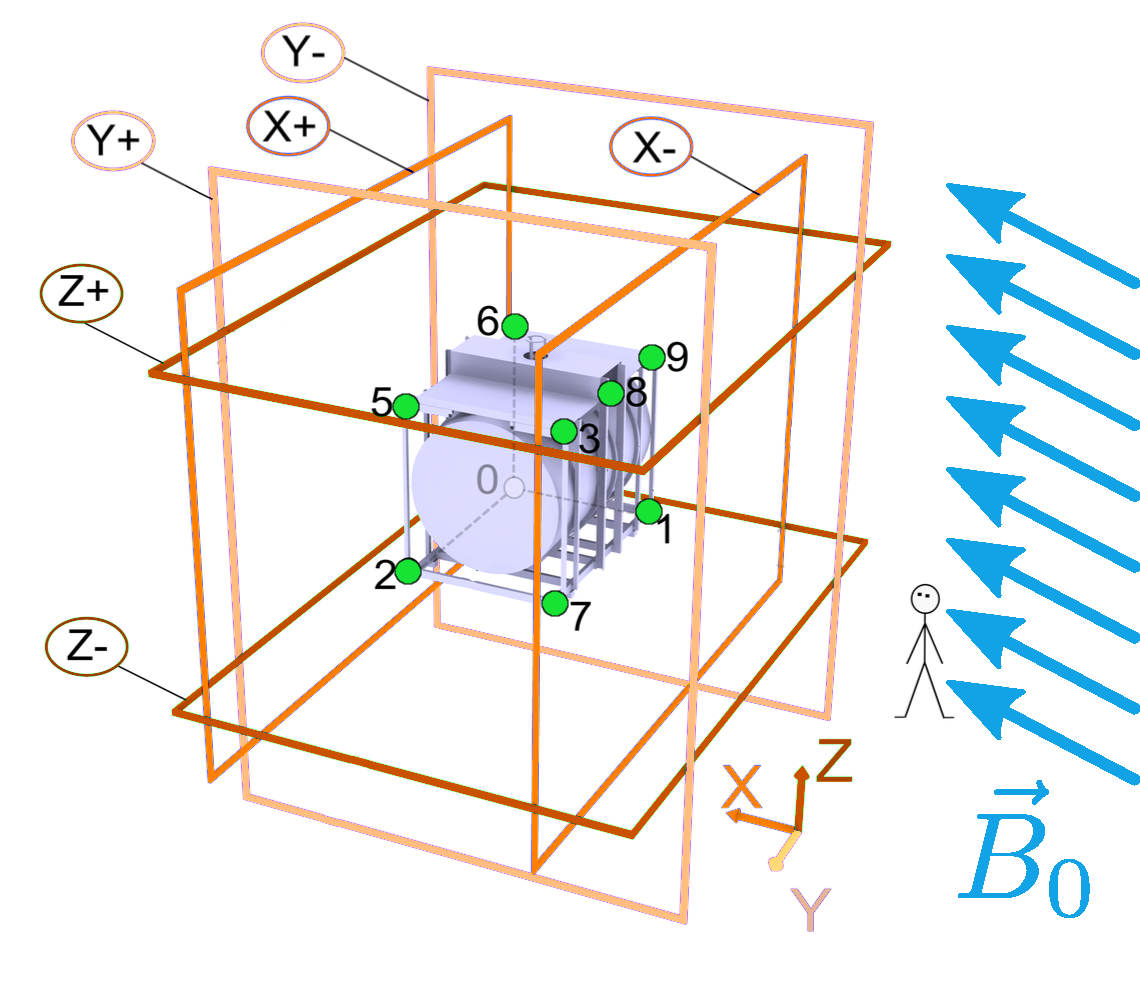
\includegraphics[width=0.8\linewidth]{gfx/nEDM_SFC/SFCplain.pdf}
  \caption{\ldots. Adapted from~\cite{Franke2013}.1}
  \label{fig:sfc-scheme}
\end{figure}

Active shields do not substitute passive ones. The shielding factor
\marginpar{Shielding factor, measured in \si{\decibel} is the ratio of the power in the magnetic field outside the shield to the one inside.} of passive shields degrades by as much as \SI{40}{\decibel} (two orders of magnitude in amplitude) for frequencies slower than \SIrange[range-phrase = --]{1}{10}{\hertz}~\cite{Brake1991}. At the same time the active systems perform best at DC and reach up to the kilohertz regime. The combination of the two provides a stable magnetic field over the whole range of frequencies~\cite{Kelha1982,Brake1991,Voigt2013}.

In the overlapping range of frequencies, where the two kinds of magnetic shielding could compete, the two advantages of the active shielding would certainly be the cost and accessibility of the enclosed volume. \note{disadvantage: the high-order changes}

Numerous active magnetic field compensation systems have been built \cite{Kelha1982,Brake1991,Spemann2003,Brys2005,Kobayashi2012,Voigt2013,Afach2014}. The last one, built for the nEDM@PSI experiment, is the focus of this chapter.


\section{The nEDM SFC system}
The construction of nEDM@PSI active magnetic field compensation system, called the SFC (Surrounding Field Compensation) system,
\marginpar{There is an inside joke that SFC really stands for SULTAN Field Compensation, SULTAN being the magnet with by far the strongest influence on the magnetic field.}
was a part of Beatrice Franke's PhD thesis~\cite{Franke2013} (later also published~\cite{Afach2014}). Thorough description of the system, as well as detailed characterisation, can be found there.

The author was responsible for maintaining the system, with the goal of gaining enough of understanding and experience to design a next generation system for the n2EDM experiment. In this section the author presents the most important information about the SFC system, repeating after~\cite{Franke2013}, and shares some of his insights. \note{Making my role clear.}

The distinct feature of the nEDM@PSI's SFC system is the use of the matrix \note{Need to find a name. In Bea's thesis referred to as ,,the matrix $M$''. Response matrix? SFC matrix?}. Consider a single coil of any shape in air. For every point in space and for every spatial component the magnetic field is proportional to the current in the coil, with a certain fixed proportionality constant. The SFC system has six coils and measures the field in nine points, three spatial components in each---27 channels. In total there are $6 \times 27 = 162$ proportionality constants, which are gathered in a matrix $M$. The matrix $M$ is a property of the active compensation system, more precisely of the geometry of the coils and sensors. \note{Mention that ferromagnetic materials, in particular $\upmu$-metal, also affect the matrix.}

\note{Maybe some nice formula here for the matrix elements?}

\begin{figure}
  \centering
  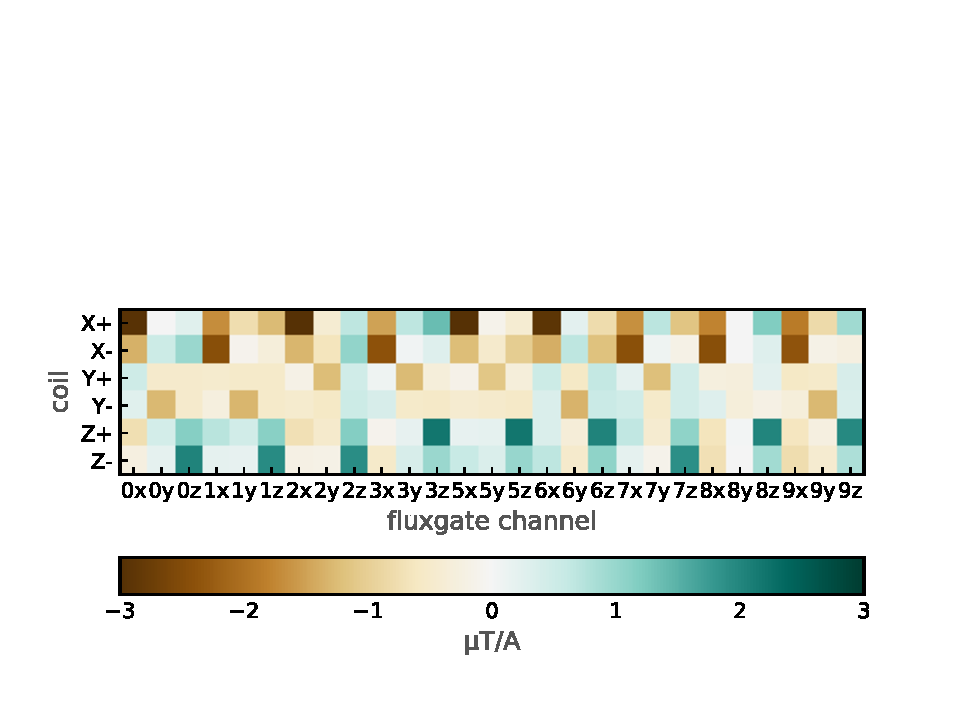
\includegraphics[width=.8\linewidth]{gfx/nEDM_SFC/nEDM_SFC_matrix}
  \caption{The SFC matrix measured by Franke on 2012-11-07 (see \cite{Franke2013}) in the thermohouse coordinates.}
  \label{fig:nEDM_SFC_matrix}
\end{figure}

The following procedure was used to measure the matrix. A current in one coil is scanned over the whole available range, while the field change is measured with the sensors. Then for each sensor, and each spatial component, a linear regression is performed. The slope is the proportionality constant (the matrix $M$ element). The procedure is repeated of all coils. The matrix measured by Franke is depicted in Fig.\,\ref{fig:nEDM_SFC_matrix}.

There is a fundamental meaning behind the matrix $M$. The currents in the six coils we can gather into a vector $\mathbb{I}$ in a space we call the \emph{current space}. Similarly, the 27 readouts of the magnetic field can be gathered into a vector $\mathbb{B}$ in the \emph{field space}. \note{think about the name}. Then the matrix $M$ provides the transition from the current into the field space. In particular, we have:
\begin{equation}
  \mathbb{B} = M \mathbb{I} + \mathbb{B}_\text{offset} \ .
\end{equation}
The other direction, from the field to the current space, cannot be done exactly. Nevertheless, the optimal, in the least-squares sense, transition can be done with the use of the Moore--Penrose inverse (pseudoinverse) \note{cite something?} of the matrix $M$, denoted $M^\dagger$.
\marginpar{Finding the pseudoinverse of a matrix $A$ is equivalent to finding least-squares solution of a system of linear equations described by the matrix $A$ (although more computationally complex).}
In other words, the matrix $M$ tells us what field, as measured by the sensors, will a given set of currents produce. The matrix $M^\dagger$ tells us what currents to apply to best approximate a given field.

The use of the matrix $M$ was what distinguished the nEDM@PSI's SFC system from other systems~\cite{Kelha1982,Brake1991,Spemann2003,Brys2005,Kobayashi2012,Voigt2013}. The others used either one component of a sensor, or a weighted combination of several components, to control one coil. The matrix was first proposed by~\cite{RetaHernandez1998}. As their proposed system did not include $\upmu$-metal, they could calculate the matrix analytically.



\section{The feedback algorithm}
In the old system the currents were controlled with a PID algorithm (as most of the previous systems, cite them)
The nEDM@PSI's SFC system followed the norm established by older systems~\cite{Kelha1982,Brake1991,Spemann2003,Brys2005} \note{may want to verify} and used a PID loop to control the currents. (PI in this particular case, the derivative term was not used.) The $j$th current in the $n$th iteration was given~\cite{Franke2013}:
\begin{equation}
  \label{eq:old_SFC_feedback}
  I^n_j = I^0_j +
    \underbrace{ \alpha^\mathcal{P}_j \, \Delta I^n_j }_\text{proportional term} +
    \underbrace{ \alpha^\mathcal{I}_j \, \sum_m \Delta I^m_j }_\text{integral term} \ .
\end{equation}

$\Delta I^n_j$ is the error value in the current space. It was obtained by using the error value in the field space (the difference of the measured and target fields) and transforming it into the current space with the pseudoinverse of the matrix:
\begin{equation}
  \Delta I^n_j = \sum_{k'} \hat{M}^{-1}_{jk'} \, \Delta B^n_{k'} \ .
\end{equation}

Besides the proportional and integral terms the feedback formula also includes the $I^0_j$ term. It seems weird to give such a big of a role to particular currents that happened to be there at the zeroth iteration. It has to do with the following property of the system: the target field was always the one measured at the moment of switching the system from dynamic to static.
\marginpar{The system when turned on was always static. Then the currents could be changed manually to achieve a desired field (or chosen from a predefined set). Then the system was switched to the dynamic mode.}
At that moment the error value was zero, and so was the integral term, so, according to the Eq.\,\ref{eq:old_SFC_feedback}, the output currents would immediately have switched to zero. In result, the system would violently destabilise. The additional term $I^0_j$ prevents that from happening.



\section{The spectrum of the SFC matrix}
\label{sec:nedm_sfc_matrix}
The SFC matrix used during the data taking of the nEDM experiment (2014, 15 and 16) is the one measured by Franke \cite{Franke2013}. The matrix not only needed to be inverted, but also additionally regularised. While it has been thoroughly discussed how to do the regularisation, the question of why was it needed at all was neither posed nor answered.

Let us elaborate on regularisation. The SFC matrix represents coefficients in a set of linear equations that need to be solved in order to determine the best currents to apply for a given goal field. As the set of equation is over--determined, the best solution is found by the least--squares, which is exactly equivalent to calculating the pseudoinverse matrix. A solution can be found reliably if the system is well--defined, i.e. the solution ,,dip'' is steep in every direction in the parameter space. If the ,,dip'' becomes a valley in some directions, the solution is not globally well--defined, although it still may be defied up to a parameter (the one pointing in the direction of the valley). We then speak of an ill--defined set of equations, or an ill--defined matrix. Regularisation helps ill--defined problem to become better, at the cost of the least--squares in the solution.


A real matrix $\mathbb{M}$ may be decomposed into $\mathbb{M} = \mathbb{U} \mathbb{S} \mathbb{V}^T$, where $\mathbb{U}$ and $\mathbb{V}$ are unitary, and $\mathbb{S}$ is diagonal. This is called the \emph{Singular Value Decomposition} (SVD). The singular values lie on the diagonal of $\mathbb{S}$, which is call the \emph{spectrum}. The spectrum of the SFC matrix is of uttermost importance. Pseudoinverting a matrix with small singular values is an ill--posed problem similar, as inverting small numbers.

One defines the \emph{condition number} of a matrix as the ratio of extreme values of its spectrum. For a matrix with a flat spectrum, all singular values equal, the condition number is 1 and the set of linear equations this matrix represents is well defined. The more they differ, the higher the condition number and the worse defined the problem is. The effect in the solution is that noise in the original matrix becomes amplified by the condition number in the pseudoinverse.

Figure~\ref{fig:nEDM_SFC_svd} presents the spectrum of the nEDM SFC matrix. First thing to note is that the condition number is $9.6 / 0.51 = 18.2$. This is a factor of 20 amplification in noise and it clearly explains why regularisation was necessary.

It is interesting to ask why. A very small singular value means that there exists a coil, or a combination thereof, which has almost 20 times smaller influence on the field then others. In figure~\ref{fig:nEDM_SFC_svd} columns are the singular values with their corresponding coil--vectors. The first three, starting from the left, are easiest to interpret. Each of them is a pair of coils configured as Helmholtz--pair, with roughly the same current, producing a homogeneous field in each of the spatial directions. The smaller singular value, or the effect on the field, in the Y direction is explained by the fact that this is the longitudinal axis of the μ-metal cylinder. The last one has also a clear interpretation -- it is all pairs configured as anti--Helmholtz, with currents flowing in the opposite directions. The magnetic field that it creates is a very complicated, high-order field. The fact, that this combination has so little influence means, that it hardly changes any solution for currents when added upon it. It spans a valley in the parameter space in the least--squares problem.

\begin{figure}
  \centering
  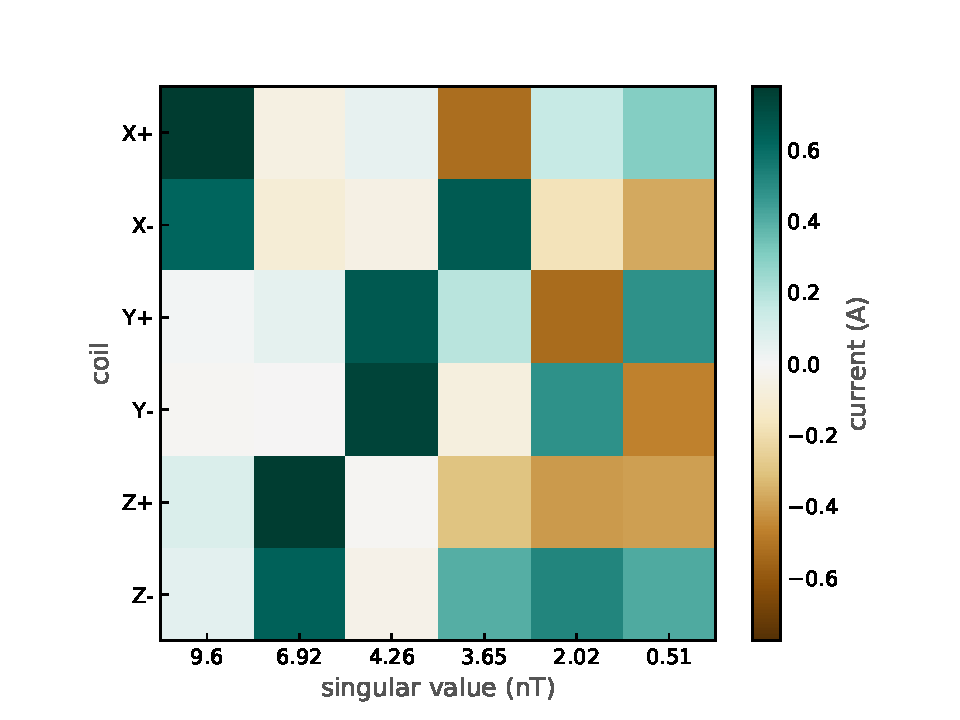
\includegraphics[width=.7\linewidth]{gfx/nEDM_SFC/coil-singular_vectors_of_the_nEDM_SFC_matrix}
  \caption
  [TODO]
  {The coil-singular values of the SFC matrix. Columns correspond to singular combinations of the coils. For each column the corresponding singular value is indicated. See text for details.}
  \label{fig:nEDM_SFC_svd}
\end{figure}

It is to note that the SFC matrix is defined solely by the configuration of the coils and sensors. It follows that care has to be taken already at the design stage to create a system that will be well defined.



\section{Visualisation of the data}
A typical question for the SFC data: I see the field changing. How does the field that induced this change look like?

Why difficult? First, the fluxgates only measured the field already compensated---the sum of the external field and the one created by SFC's coils. Three dimensional field in a three dimensional space. The field is deformed by the $\upmu$-metal shield. And the interesting field is often relative (magnet ramped, its field is the difference between after and before the ramp).

The solution was to create an interactive tool to visualise and explore the SFC data.

\begin{figure}
  \centering
  \subfloat[Displaying the calculated back external field, the movable yellow cursor chooses the data to be displayed in the 3D view.]{
    \label{fig:nEDM_SFC_visualisation1}
    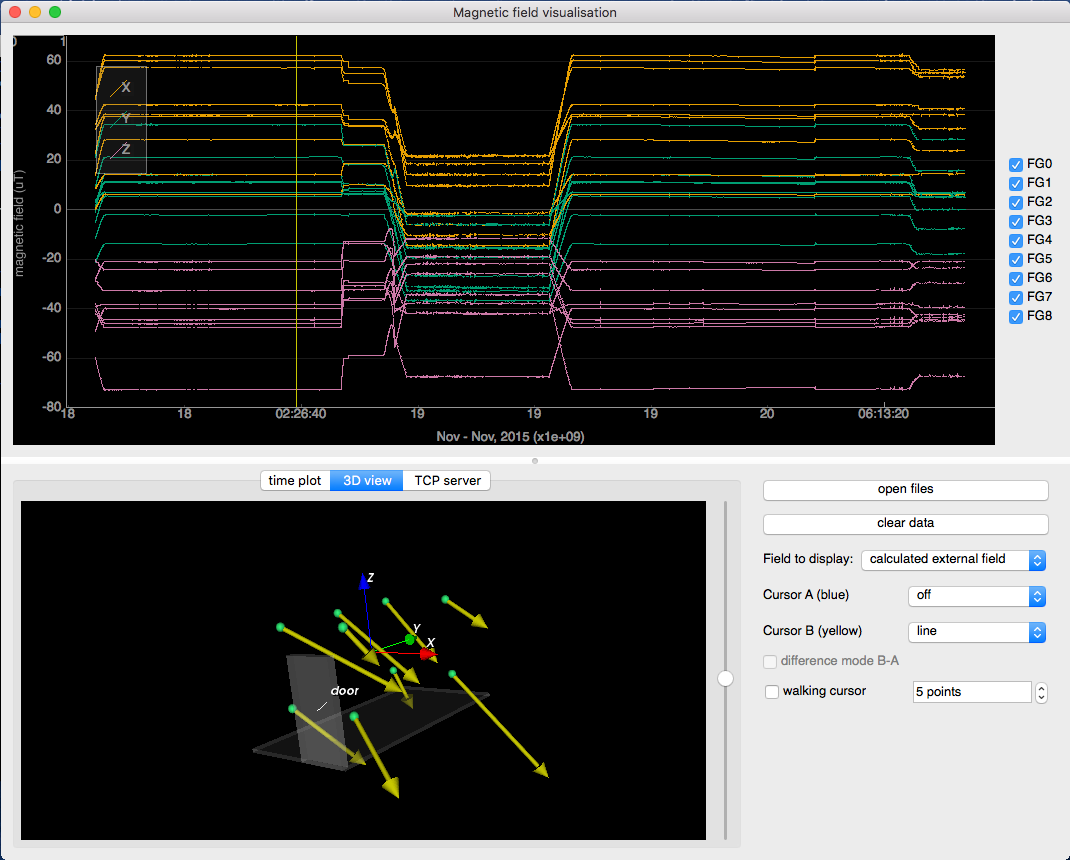
\includegraphics[width=.45\linewidth]{gfx/nEDM_SFC/visualisation/visualisation1}}
  \quad
  \subfloat[Displaying fields at two different times simultaneously, yellow and blue.]{
    \label{fig:nEDM_SFC_visualisation2}
    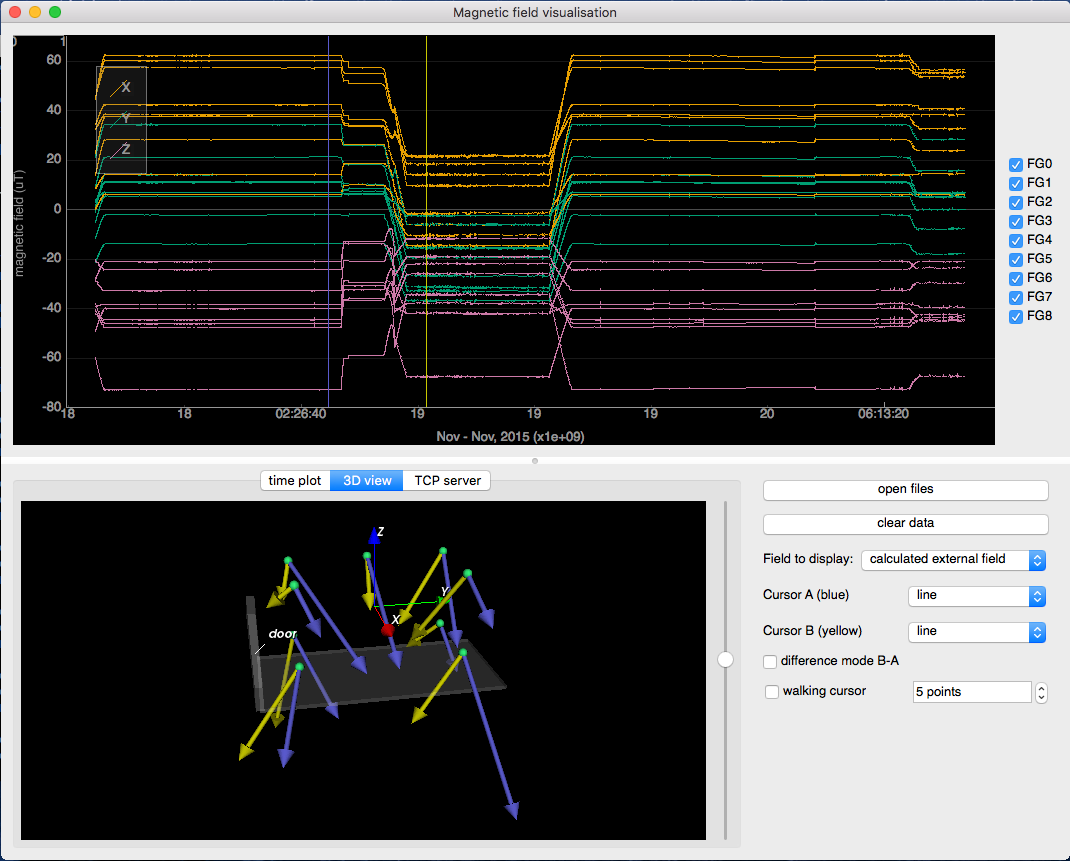
\includegraphics[width=.45\linewidth]{gfx/nEDM_SFC/visualisation/visualisation2}}
  \\
  \subfloat[Displaying a range of data, marked with the yellow cursor, relative to the point marked with the blue cursor. The calculated back external magnetic field is displayed.]{
    \label{fig:nEDM_SFC_visualisation3}
    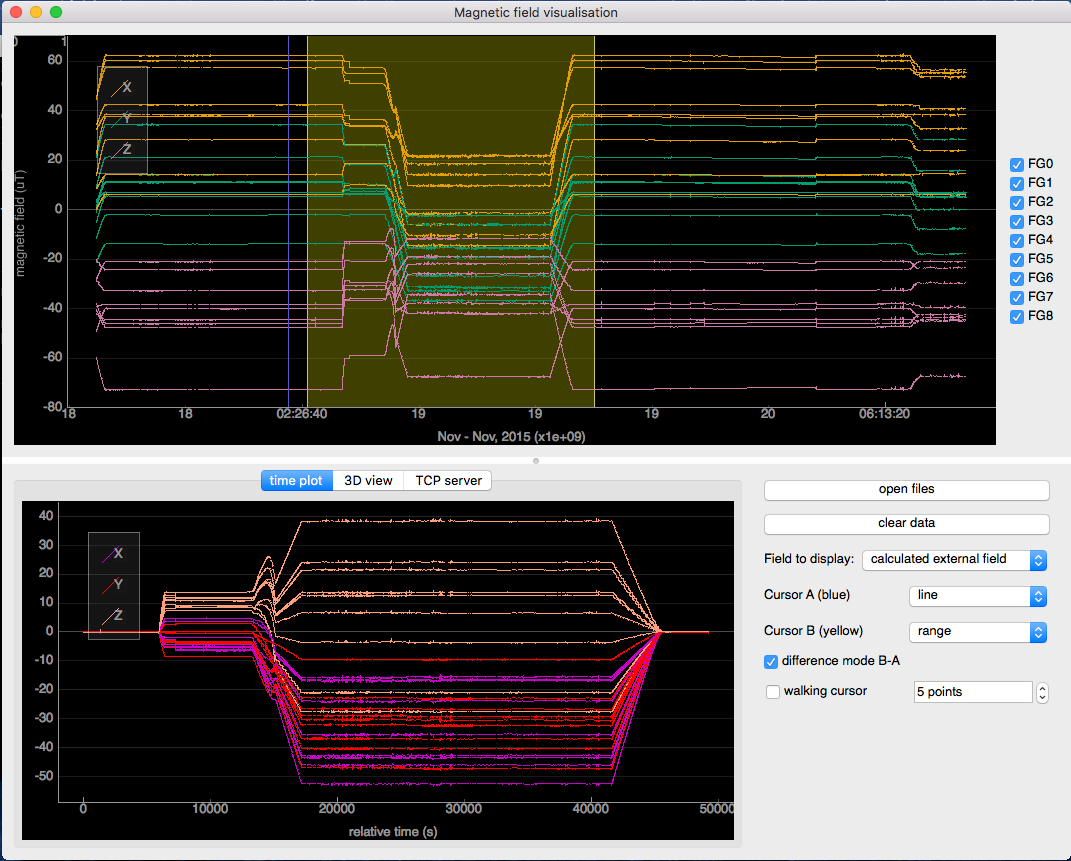
\includegraphics[width=.45\linewidth]{gfx/nEDM_SFC/visualisation/visualisation3}}
  \quad
  \subfloat[Displaying the difference between the external field in two points in geometrical form.]{
    \label{fig:nEDM_SFC_visualisation4}
    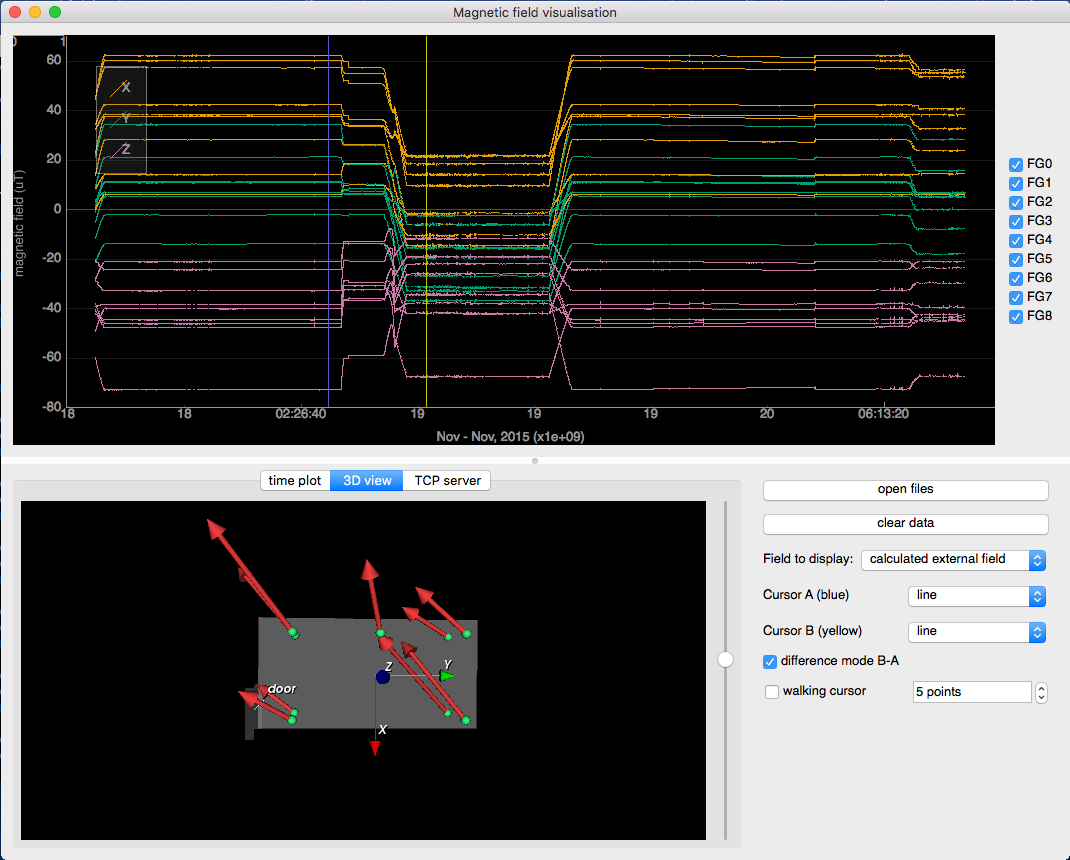
\includegraphics[width=.45\linewidth]{gfx/nEDM_SFC/visualisation/visualisation4}}
  \caption{Different functionalities of the nEDM SFC data visualisation tool.}
\end{figure}

The overview can be seen in Fig.\,\ref{fig:nEDM_SFC_visualisation1}. There are two plot areas, upper in the time domain, lower can be switched between a 3D geometrical representation and a second time-domain plot. The loaded set of data, spanning 18-20 Nov 2015, shows a ramp of the SULTAN magnet. The ,,field to display'' setting is set to ,,calculated external field'', given by:
\begin{equation}
  \mathbb{B} - \mathbb{M} \mathbb{I}
\end{equation}
Another option is displaying the measured field $\mathbb{B}$.
In the first part the field points in the $x$ direction (North) and 45 degrees downwards (Villigen is 47 degrees in latitude). As expected for the Earth's magnetic field. On the upper plot there is a vertical yellow line, a movable cursor, that chooses which point in time is depicted in the 3D visualisation. There it visualises what is more-or-less the Earth's magnetic field at the experiment's position.

In Fig.\,\ref{fig:nEDM_SFC_visualisation2} two cursors, blue and yellow, are used simultaneously to juxtapose the ,,calculated external field'' before and after the ramp. In Fig.\,\ref{fig:nEDM_SFC_visualisation3} the ,,difference mode B-A'' has been turned on. In the bottom plot we observe the SULTAN ramp relative to the field before the ramp. This is the field of the magnet as seen in the experiment site. In Fig.\,\ref{fig:nEDM_SFC_visualisation4} this field is visualised graphically, pointing South-East.

\note{Maybe show the field of COBRA, too!}

The program is cross--platform (Windows, OSX, Linux), fully based on open--source softwore. It is written in python and uses the following libraries: Qt4 (cross-platform GUI), pyqtgraph (fast interactive plotting), VTK (3D graphics) and SciPy (data handling). It is a joint work with Nils Ebeling, for whom it was a summer project.

Although it is very technical, it is very easy to underestimate the role of having data exploration tools at hand while the experiment is running.



\section{Performance during SULTAN ramps}
Another task was to compare the SFC performance in shielding SULTAN ramps in 2015 and 2016. From a rather quick look at the data it seemed that the field inside the apparatus, as seen by the Hg comagnetometer and Cs magnetometers, was affected more strongly by the ramps in 2016 than in 2015.

% ((ext_field - B_Earth) * B_SULTAN)
The first is to determine the times of the ramps. Unfortunately, those data are not easily available. But could be calculated from the SFC data.

We define $\mathbb{B}_\text{Earth}$ as the uncompensated field ($\mathbb{B} - \mathbb{M} \mathbb{I}$) when the SULTAN magnet is known to be off. We then define the field of the SULTAN magnet to be $\mathbb{B}_\text{SULTAN} = \mathbb{B} - \mathbb{M} \mathbb{I} - \mathbb{B}_\text{Earth}$, when the magnet was known to be on. Then we can calculate the content of the SULTAN in the field by projecting the uncompensated field, minus the Earth's, on the one of the SULTAN:
\begin{equation}
  \left( \mathbb{B} - \mathbb{M} \mathbb{I} - \mathbb{B}_\text{Earth} \right) \cdot \mathbb{B}_\text{SULTAN}  
\end{equation}

\begin{figure}
  \centering
  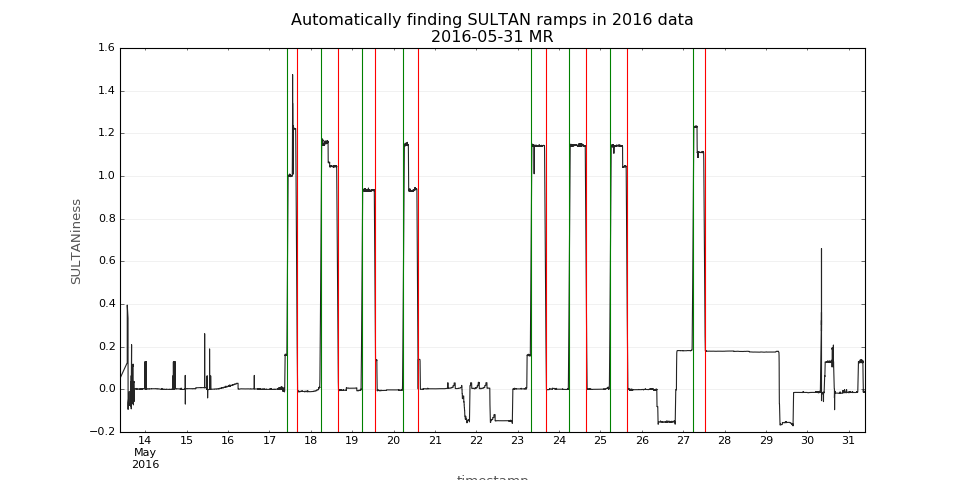
\includegraphics[width=.7\linewidth]{gfx/nEDM_SFC/finding_SULTAN_ramps.png}
  \caption
  [TODO]
  {\ldots}
  \label{fig:finding_SULTAN_ramps}
\end{figure}

The value of this projection for two weeks in May 2016 is depicted in Fig.\,\ref{fig:finding_SULTAN_ramps}. The SULTAN ramps are wonderfully pronounce and their times easy to get, as the times when the projection crosses 0.5 going up (ramp up) or down (ramp down).

\begin{figure}
  \centering
  \subfloat[Displaying the calculated back external field, the movable yellow cursor chooses the data to be displayed in the 3D view.]{
    \label{fig:SULTAN_ramp_Hg_performance}
    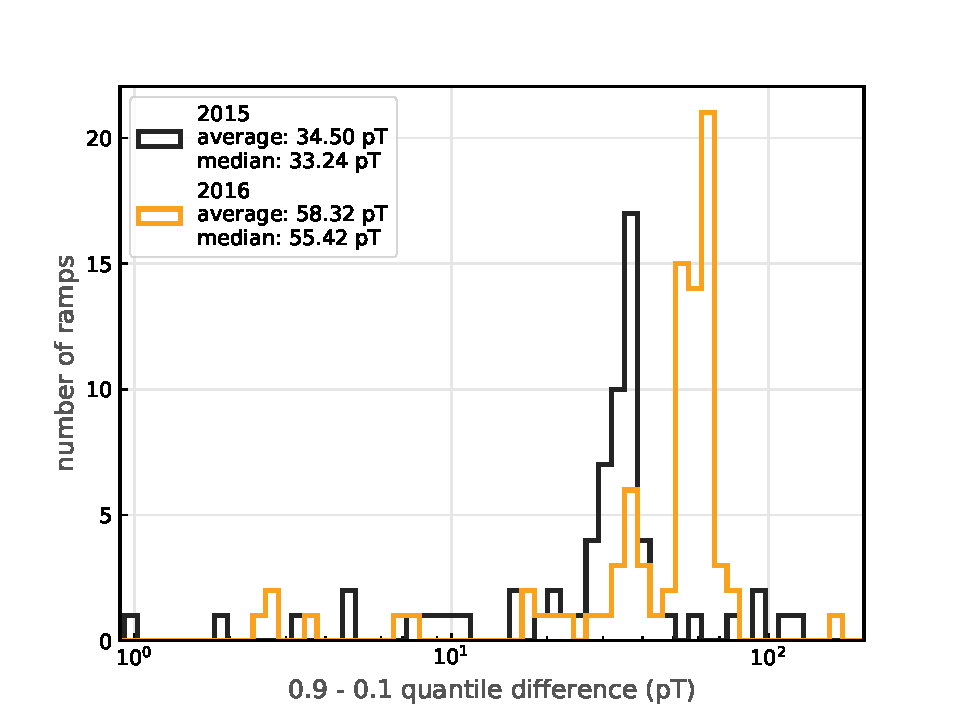
\includegraphics[width=.45\linewidth]{gfx/nEDM_SFC/field_seen_by_Hg_2015-2016}}
  \quad
  \subfloat[Displaying fields at two different times simultaneously, yellow and blue.]{
    \label{fig:SULTAN_ramp_Cs_performance}
    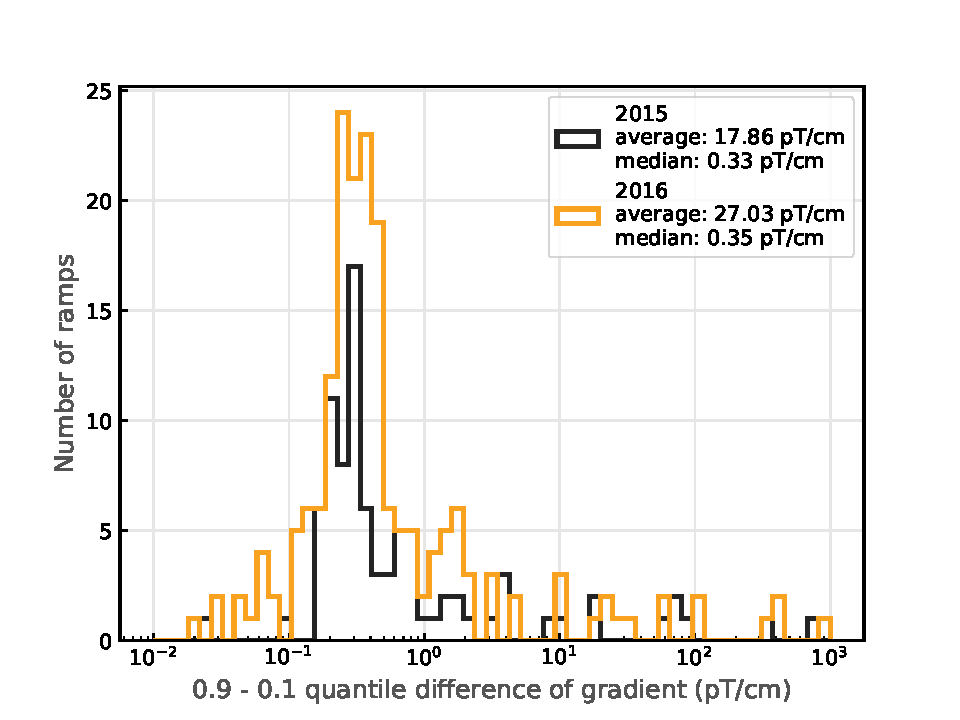
\includegraphics[width=.45\linewidth]{gfx/nEDM_SFC/gradient_seen_by_Cs_2015-2016}}
  \caption{Magnetic field of the SC magnet seen by the SFC. Taken as difference of runs...}
\end{figure}

With the exact times of the SULTAN ramps available, the Hg comagnetometer and Cs magnetometer data in a 2h window around each of the ramps were taken. From the Cs data the gradient was estimated as the difference between the averages of the top and bottom sensors, divided by the separation of \SI{25.1}{\centi\meter}. The change was defined as 0.9 and 0.1 quantile difference. The histogram for all the field changes, as measured by the Hg, during SULTAN ramps is shown in Fig.\,\ref{fig:SULTAN_ramp_Hg_performance}. It is visible that while in 2015 the changes are consistently around \SI{34}{\pico\tesla}, in 2016 the changes are centred around \SI{55}{\pico\tesla}.

\note{Look once again into the data, try to see what the peak is.}

\note{Write that the scheme may be more generally used?}

Conclusion: reason is unknown, but the incentive to find it out is not to strong. Changes in the field are compensated by the Hg magnetometer. The uncompensated vertical gradient change remained the same.






% \section{Influence of the SC magnet}
% The ultracold neutrons are polarised by passing through a superconducting magnet. The length of the path of the neutrons to the experiment should be small to minimise transport losses. For this reason the experiment is located close to the exit of the UCN beam--port and the magnet is fit in between.

% \begin{figure}
%   \centering
%   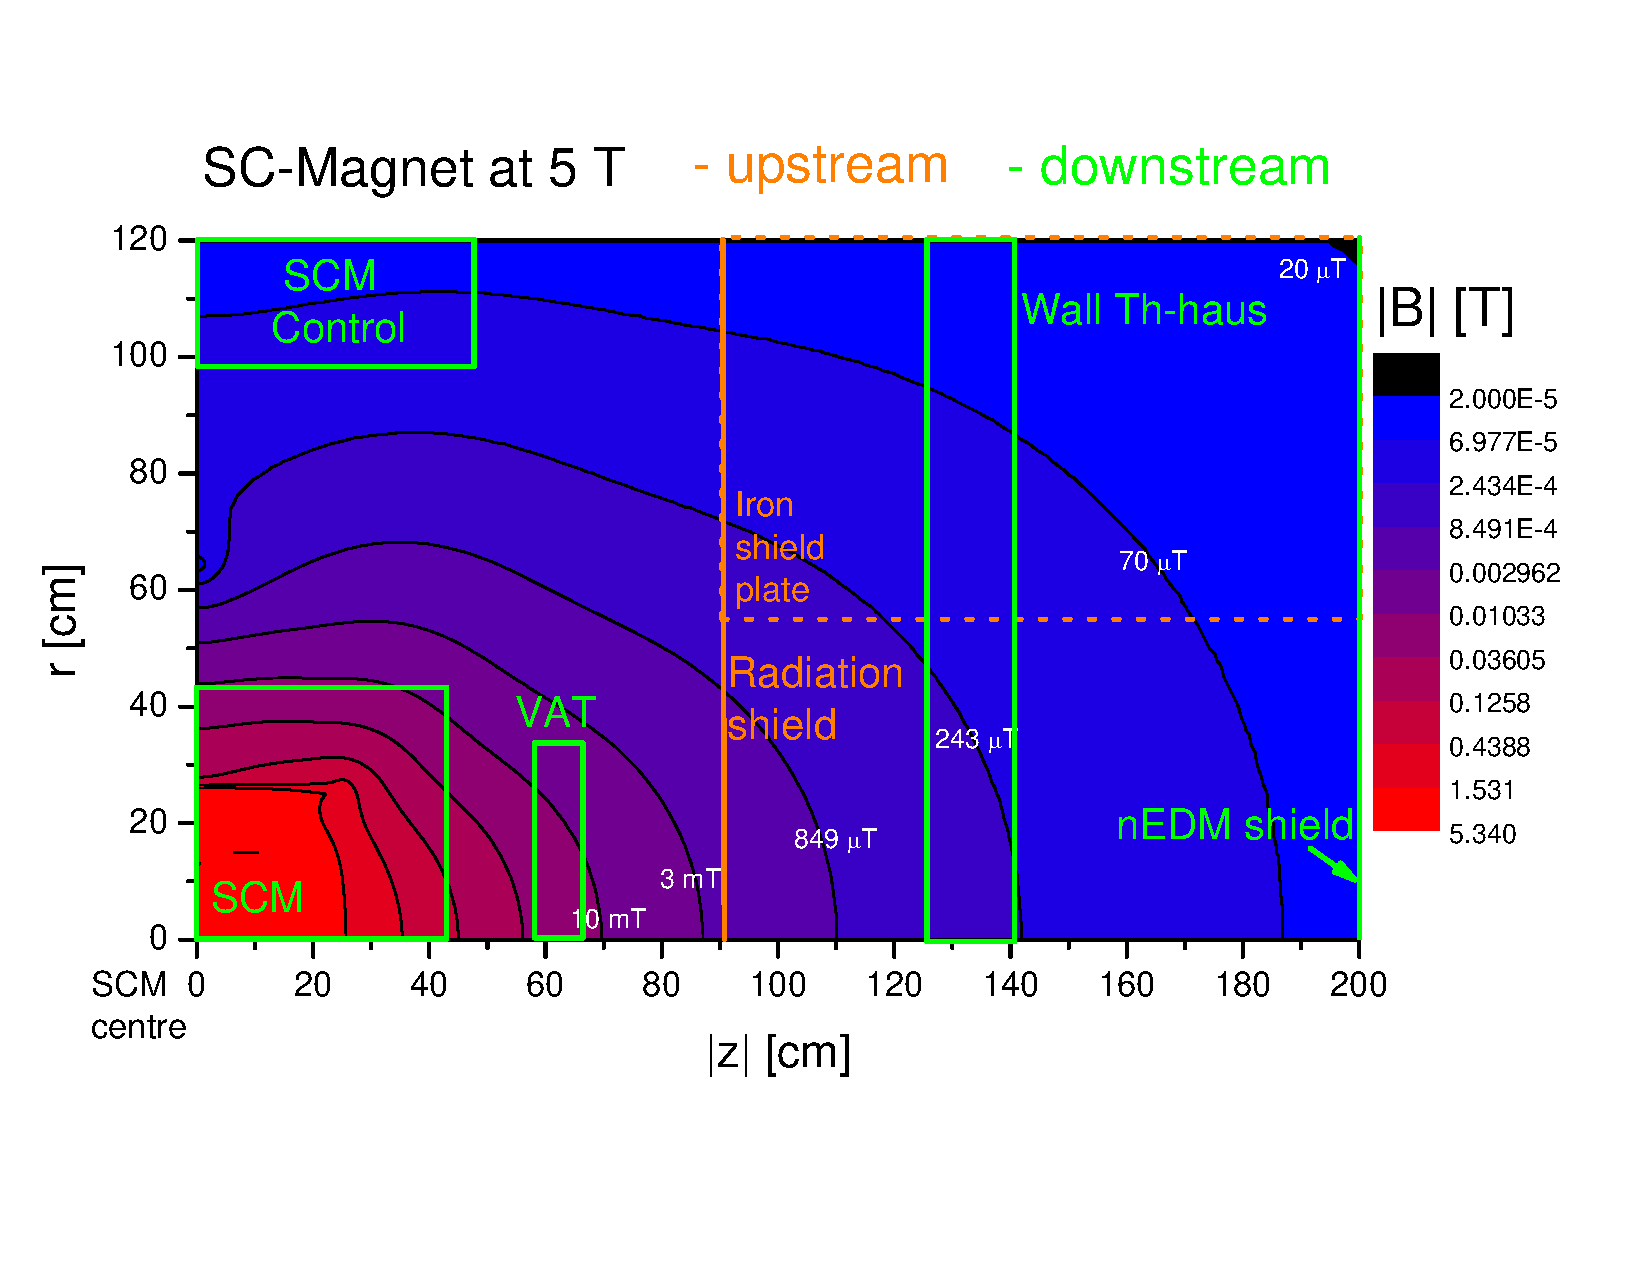
\includegraphics[width=.7\linewidth]{gfx/nEDM_SFC/SCM_magn_map.pdf}
%   \caption
%   [TODO]
%   {Map of the magnetic field of the superconducting magnet. Courtesy of Dr. Geza Zsigmond}
%   \label{fig:nEDM_SFC_SC_magnet_map}
% \end{figure}

% \begin{figure}
%   \centering
%   \subfloat[Displaying the calculated back external field, the movable yellow cursor chooses the data to be displayed in the 3D view.]{
%     \label{fig:nEDM_SFC_SC_magnet_influence_top_view}
%     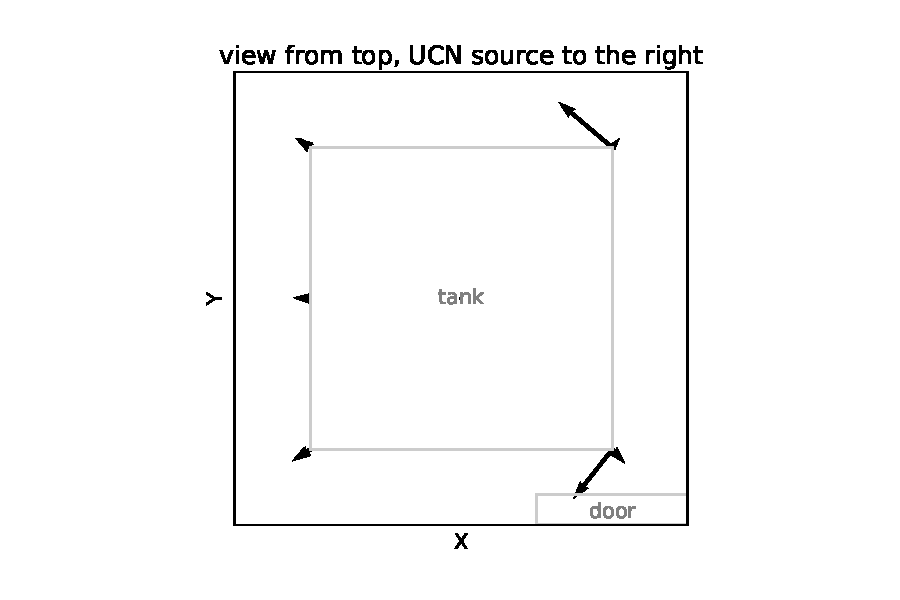
\includegraphics[width=.45\linewidth]{gfx/nEDM_SFC/SC_magnet_field_top_view.pdf}}
%   \quad
%   \subfloat[Displaying fields at two different times simultaneously, yellow and blue.]{
%     \label{fig:nEDM_SFC_SC_magnet_influence_front_view}
%     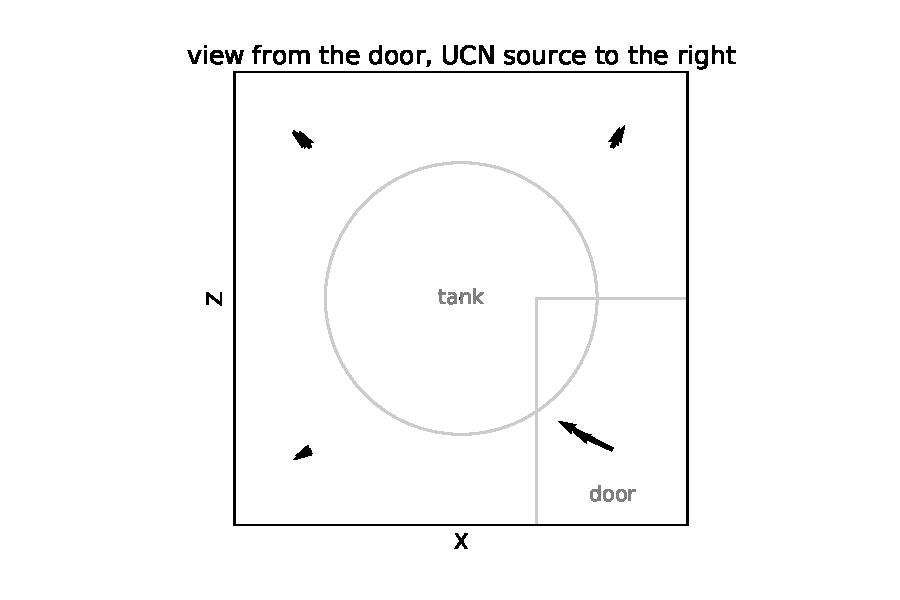
\includegraphics[width=.45\linewidth]{gfx/nEDM_SFC/SC_magnet_field_front_view.pdf}}
%   \caption{Magnetic field of the SC magnet seen by the SFC. Taken as difference of runs...}
% \end{figure}

% \begin{figure}
%   \centering
%   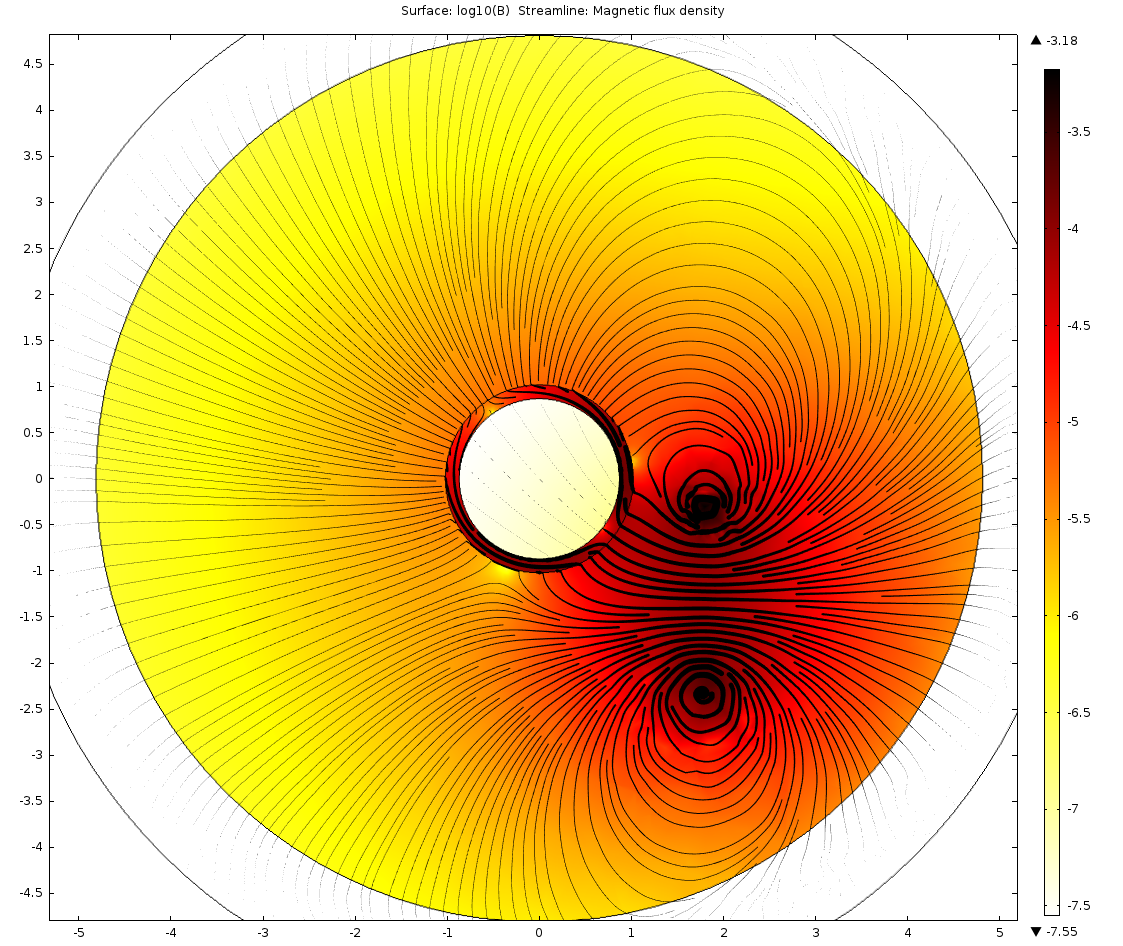
\includegraphics[width=.7\linewidth]{gfx/nEDM_SFC/SC_magnet_optimal_coil_on_wall.png}
%   \caption
%   [TODO]
%   {Map of the field of a potential correcting coil}
%   \label{fig:nEDM_SFC_SC_magnet_optimal_coil}
% \end{figure}

% \begin{figure}
%   \centering
%   \subfloat[Displaying the calculated back external field, the movable yellow cursor chooses the data to be displayed in the 3D view.]{
%     \label{fig:nEDM_SFC_SC_magnet_influence_top_view2}
%     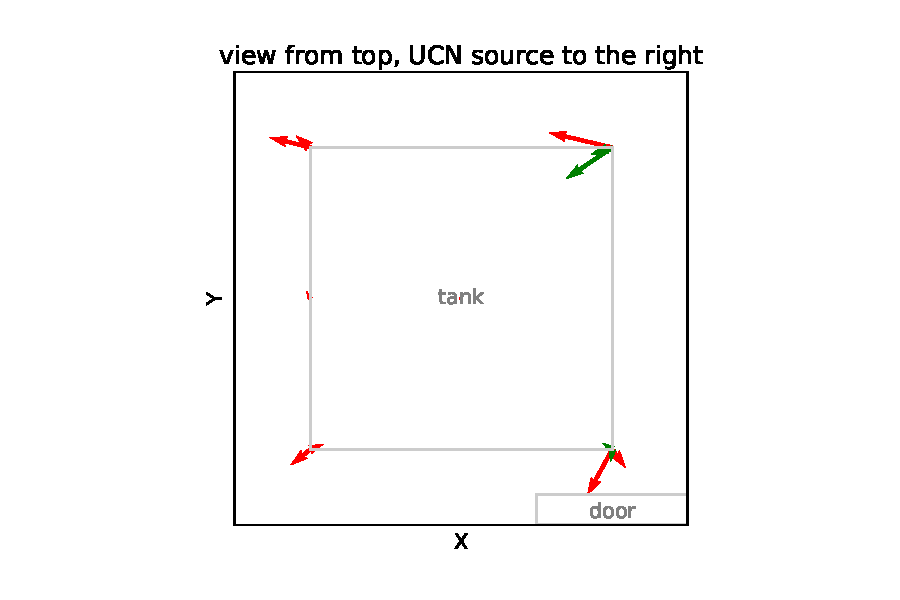
\includegraphics[width=.45\linewidth]{gfx/nEDM_SFC/SC_magnet_improvement_top_view.pdf}}
%   \quad
%   \subfloat[Displaying fields at two different times simultaneously, yellow and blue.]{
%     \label{fig:nEDM_SFC_SC_magnet_influence_front_view2}
%     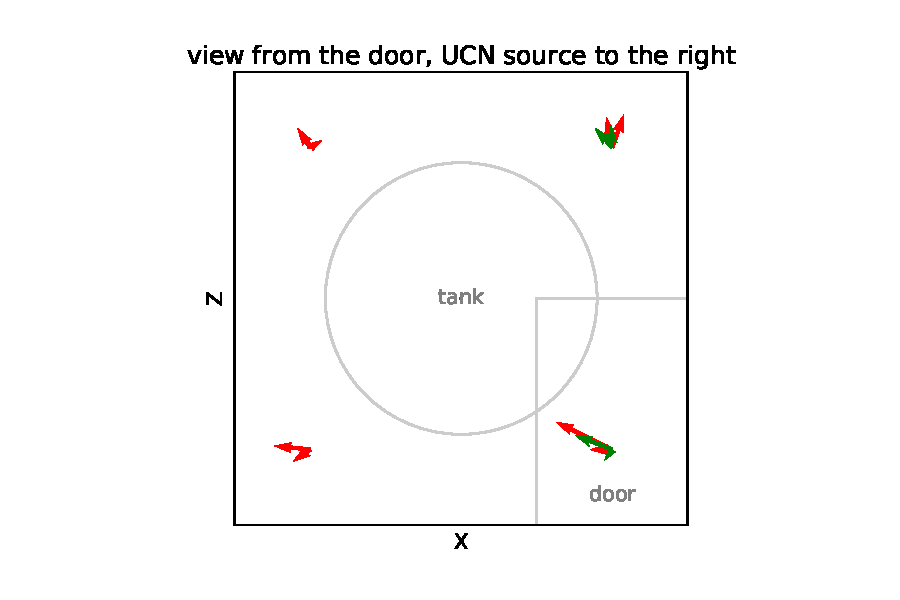
\includegraphics[width=.45\linewidth]{gfx/nEDM_SFC/SC_magnet_improvement_front_view.pdf}}
%   \caption{Magnetic field of the SC magnet seen by the SFC. Taken as difference of runs...}
% \end{figure}

% The improvement in the range of the field is 40-70\% (In different simulated runs, 21.7 to 12.6 (42\%), 22.2 to 12.9 (42\%), 19.3 to 5.8 (70\%), and 35.1 to 18.6 (57\%)), unit microteslas.


\section{Magnetic field during sparks in HV}

This is important! As clearly the most dangerous magnetic fields are ones correlated with HV.


\begin{figure}
  \centering
  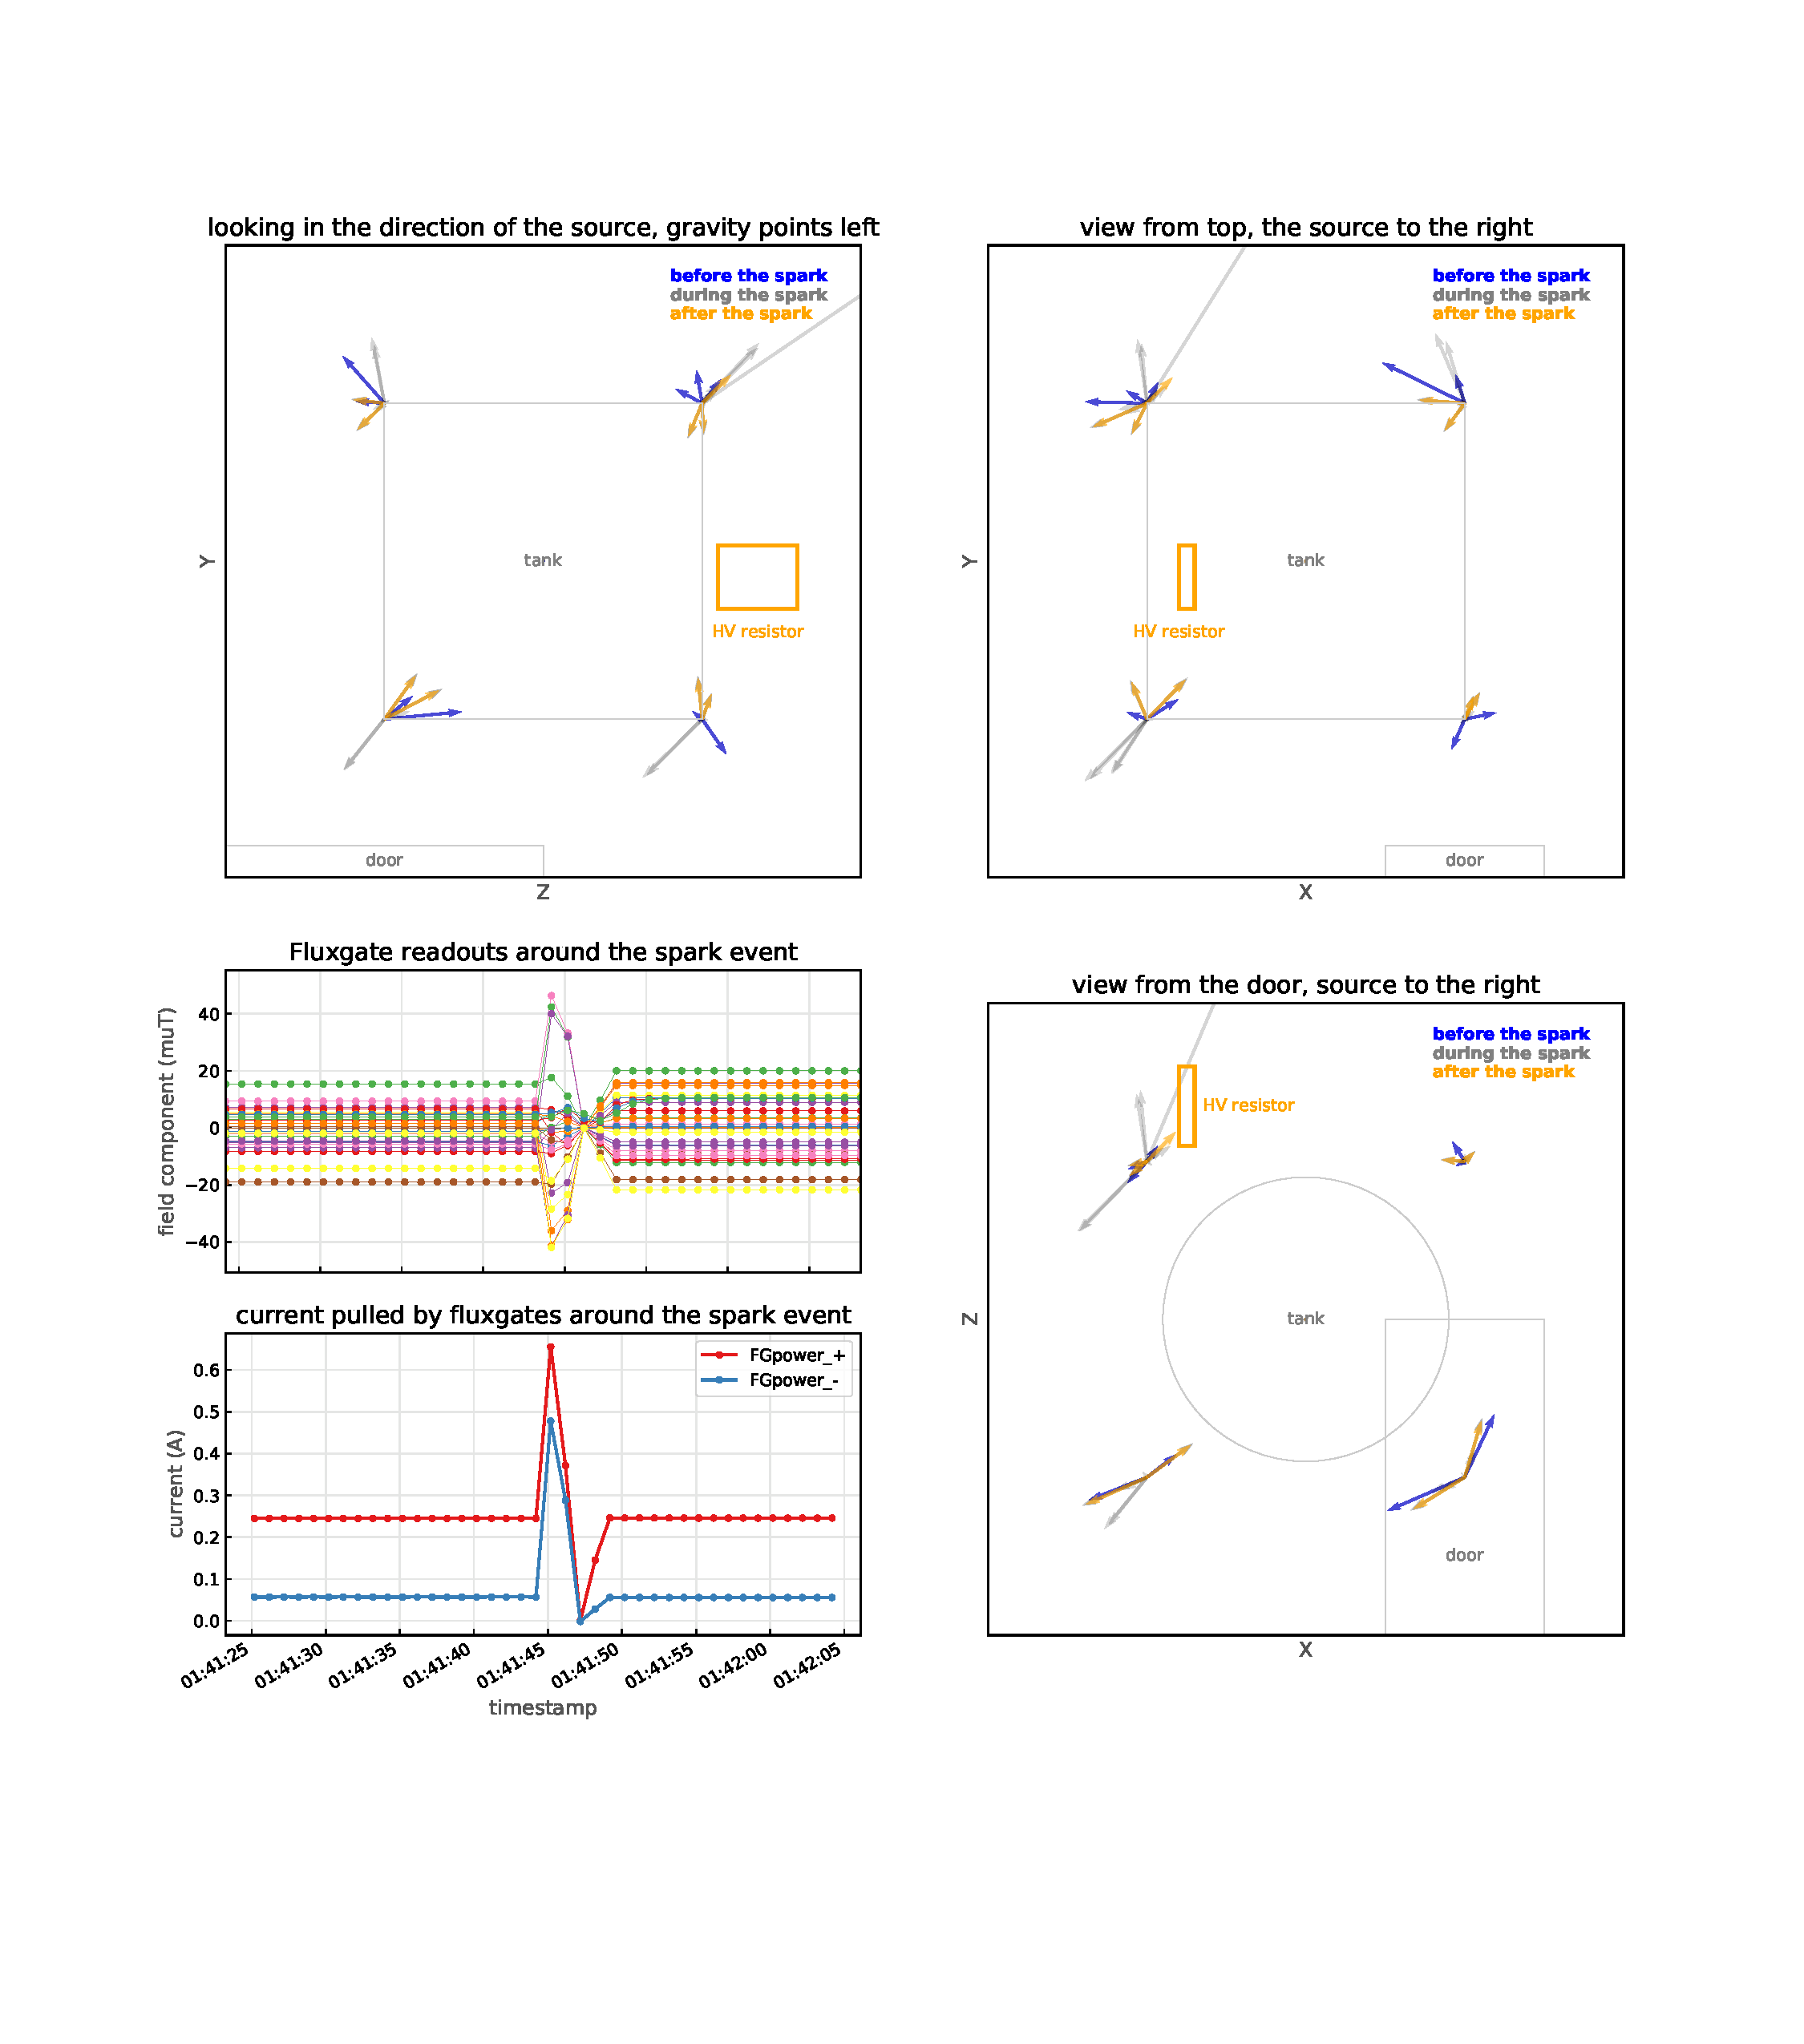
\includegraphics[width=.7\linewidth]{gfx/nEDM_SFC/SFC_during_spark_event_thesis.pdf}
  \caption
  [TODO]
  {\ldots}
  \label{fig:field_when_sparking}
\end{figure}









\section{Optimising the number of windings in the coils}
Put the plots of the distributions of the currents, juxtapose them with the
ranges of the power supplies.






\section{Remote magnetometers}
Write the documentation, show a SULTAN ramp as seen by the magnetometers, boast a bit about the automatic deployment, timing accuracy and so on.

Work of Gianluca Janka and Hanno Bertle.
